\chapter{Testování softwaru}
Cílem testování softwaru je zjištění kvality daného softwaru, zda splňuje veškeré smluvené nároky například na výkonnost nebo správnost řešení a pomáhá odhalovat chyby. Testování je nedílnou součástí vývoje SW, obvykle se software či jeho části testují průběžně. A to především z důvodu včasného odhalení chyb, které je možné v průběhu vývoje snáze opravit. Testování softwaru může sloužit jako prostředek k mitigaci rizik, cílem je snížení či eliminace rizik spojených s nasazením chybného kódu do produkčního prostředí.

\section{Historie testování}
První chyba či selhání celého počítače bylo zaznamenáno v padesátých letech 20. století na Harvardově univerzitě. Chyba však nestála na straně softwaru, nýbrž příčinou byla zaklíněná můra v součástkách tehdejšího sálového počítače s označením Mark II, a ten vypověděl službu. Z tohoto prostého důvodu se dnes při řeči o chybách v programu využívá označení „moucha“ či „bug“. Prvotně toto označení použil Thomas Edison v jeho publikacích z 19. století, nyní však šlo o první počítačovou chybu. 

Chyba v programu vede k selhání softwaru. Záznam o této chybě vzniknul v roce 1945. Podařilo se dochovat i onu můru, tedy strůjce celého problému \cite{85SxcMZY6LKfV8v4}. Kopie tohoto záznamu se nachází na obrázku \ref{fig:zaznam-o-prvni-chybe}.


\begin{figure}[!h]
	\centering
	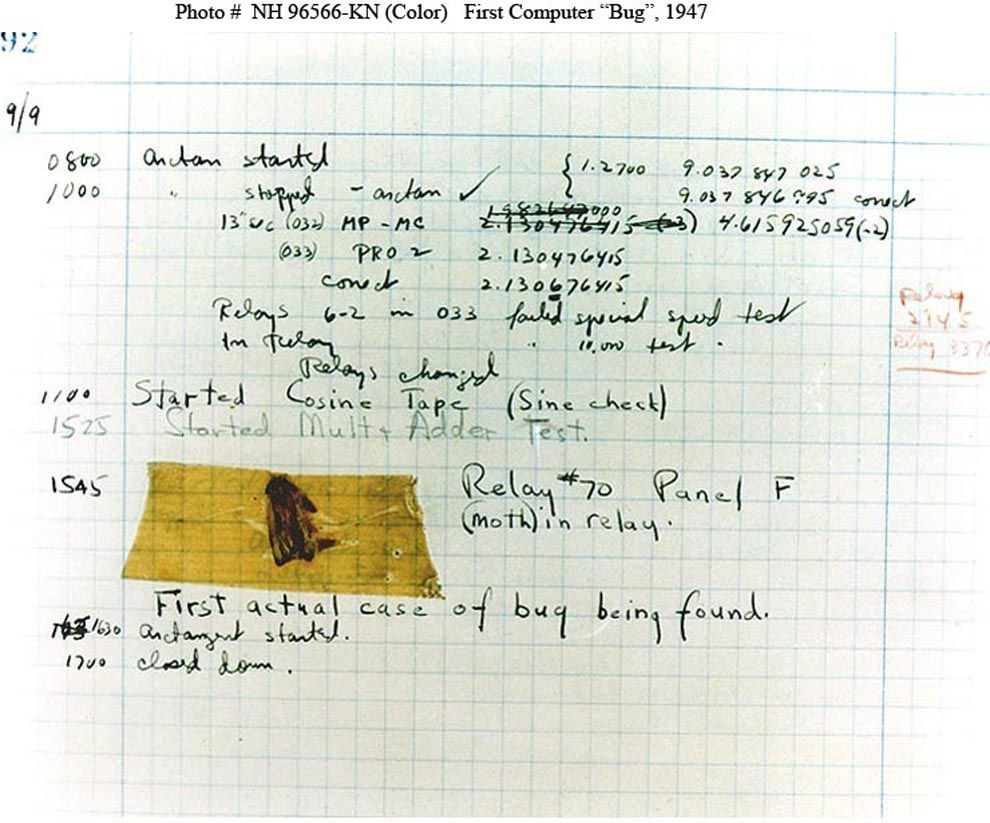
\includegraphics[width=0.5\textwidth]{Figures/first-pc-bug.jpg}
	\caption{Záznam o první počítačové chybě \cite{85SxcMZY6LKfV8v4}}
	\label{fig:zaznam-o-prvni-chybe}
\end{figure}

\section{Proces vývoje softwaru}
Mezi základní modely popisující proces vývoje softwaru patří model velkého třesku, model „programuj a opravuj“, vodopádový model nebo spirálový model. Mezi stěžejní body propracovanějších modelů se řadí specifikace, vývoj a testování. Každý tým vyvíjející software si může tento proces definovat tak, aby byl efektivní a splňoval očekávané podmínky zadavatele. Metodika či proces vývoje softwaru obvykle kombinuje hned několika principů z výše vyjmenovaných modelů. Především se však proces ubírá směrem iteračního vývoje softwaru. Vývoj softwaru v iteracích či cyklech vychází z praktických zkušeností především z důvodu přicházejících změn či doplňování specifikací už při vývoji softwaru.

Velmi důležitým krokem celého procesu vývoje softwaru je testování. Testování slouží především k odhalování chyb, které mohly být při vývoji zaneseny do kódu, a na první pohled nemusí být jasné, že se v kódu tyto chyby nacházejí. Proto je hned několik principů, jak software testovat. Metodiky testování se liší u různých projektů, a z praxe je zřejmé, že i přes sebelepší postup při testování softwaru je možné, že se chyba objeví až při užívání aplikace zákazníkem (obecně uživatelem). Cílem testování je minimalizace možnosti objevení chyb až ve fázi, kdy aplikaci využívá koncový uživatel. Některé testy či testové sady je možné automatizovat a zefektivnit tak fázi testování.

\subsection{Model velkého třesku}
Metoda vývoje, při které se využívá modelu velkého třesku stojí, na jednoduchosti celého konceptu. Veškeré úsilí je soustředěno na vývoj softwaru – konečného produktu. Model počítá s velmi nízkou úrovní specifikace výsledného softwaru. Součástí tohoto modelu není fáze formálního tetování \cite{Patton2002}. Model je vyobrazen na obrázku \ref{fig:big-bang-model}.


\begin{figure}[!h]
	\centering
	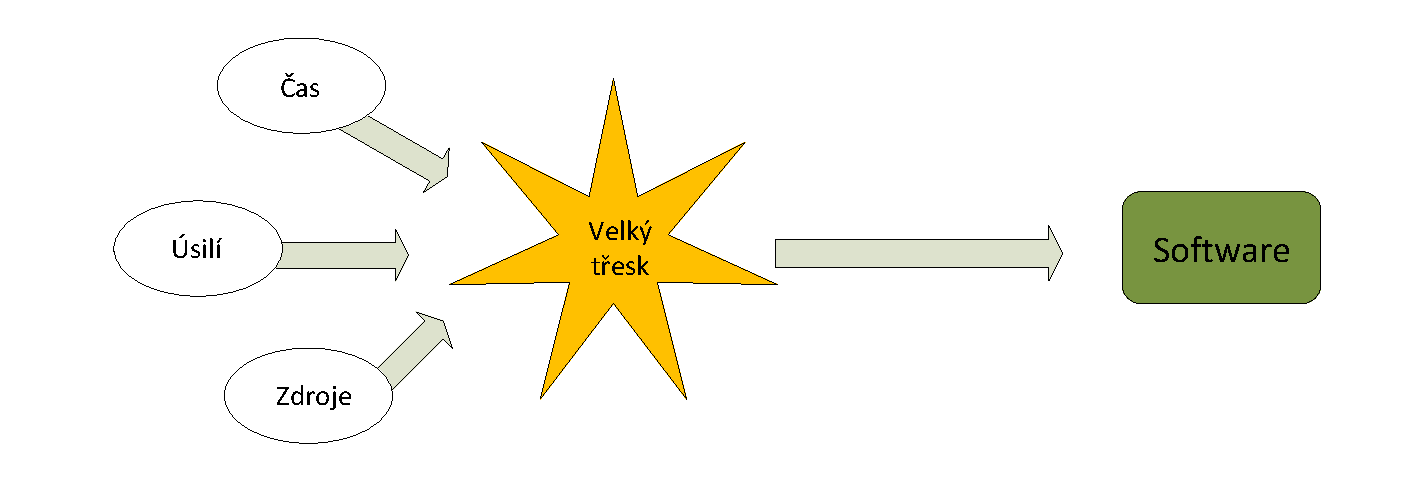
\includegraphics[width=0.8\textwidth]{Figures/VelkyTresk.pdf}
	\caption{Model velkého třesku}
	\label{fig:big-bang-model}
\end{figure}
\newpage
\subsection{Model „programuj a opravuj“}
Tento model nevyžaduje příliš mnoho režie či řízení. Je určen pro malé projekty vyžadující prezentaci výsledků v rychlém sledu. Začíná se hrubou představou o finálním softwaru, pokračuje cykly vývoje, testování a opravou chyb. Po několika iteracích těchto cyklů je rozhodnuto o ukončení práce \\a vydání softwaru. Model „programuj a opravuj“ se v praxi využívá např. u prototypů \cite{Patton2002}. Model je vyobrazen na obrázku \ref{fig:program-and-repair-model}.


\begin{figure}[h]
	\centering
	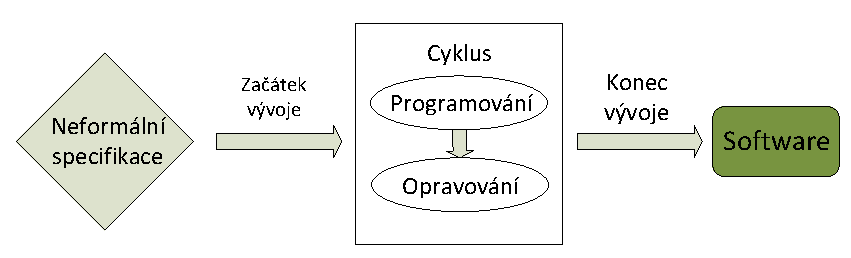
\includegraphics[width=0.8\textwidth]{Figures/ProgramujOpravuj.pdf}
	\caption{Model „programuj a opravuj“}
	\label{fig:program-and-repair-model}
\end{figure}

\subsection{Vodopádový model}
Vodopádový model spočívá v kontinuálním vývoji s přesně danou specifikací. Jednotlivé kroky tohoto modelu jsou atomické, nepřekrývají se a „není cesty zpět“. V jednotlivých krocích není možné postupovat zpětně, musí se dokončit daná iterace a začít specifikací znova \cite{Patton2002}. Model je vyobrazen na obrázku \ref{fig:waterfall-model}.

\begin{figure}[!h]
	\centering
	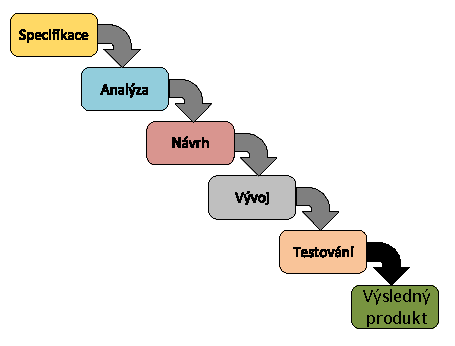
\includegraphics[width=0.5\textwidth]{Figures/waterfall.pdf}
	\caption{Vodopádový model}
	\label{fig:waterfall-model}
\end{figure}
\newpage

\subsection{Spirálový model}
Spirálový model řeší nedostatky výše uvedených modelů. Vývoj softwaru, který se řídí postupem daným spirálovým modelem je efektivní. Nevýhodou může být podstatně větší režie, než tomu bylo u modelů jako je model velkého třesku či model vodopádový. Jednotlivé kroky ve spirálovém modelu se mohou na rozdíl od vodopádového modelu překrývat \cite{Patton2002}.

V modelu jsou patrné 4 skupiny akcí, které je třeba provádět. Jmenovitě se jedná o plánování, analýzu rizik, vývoj a zhodnocení. Vývoj podle tohoto modelu probíhá v iteracích, při každém průchodu cyklem je pomyslně dokončena další část spirály. Model je vyobrazen na obrázku \ref{fig:spiral-model}.


\begin{figure}[!h]
	\centering
	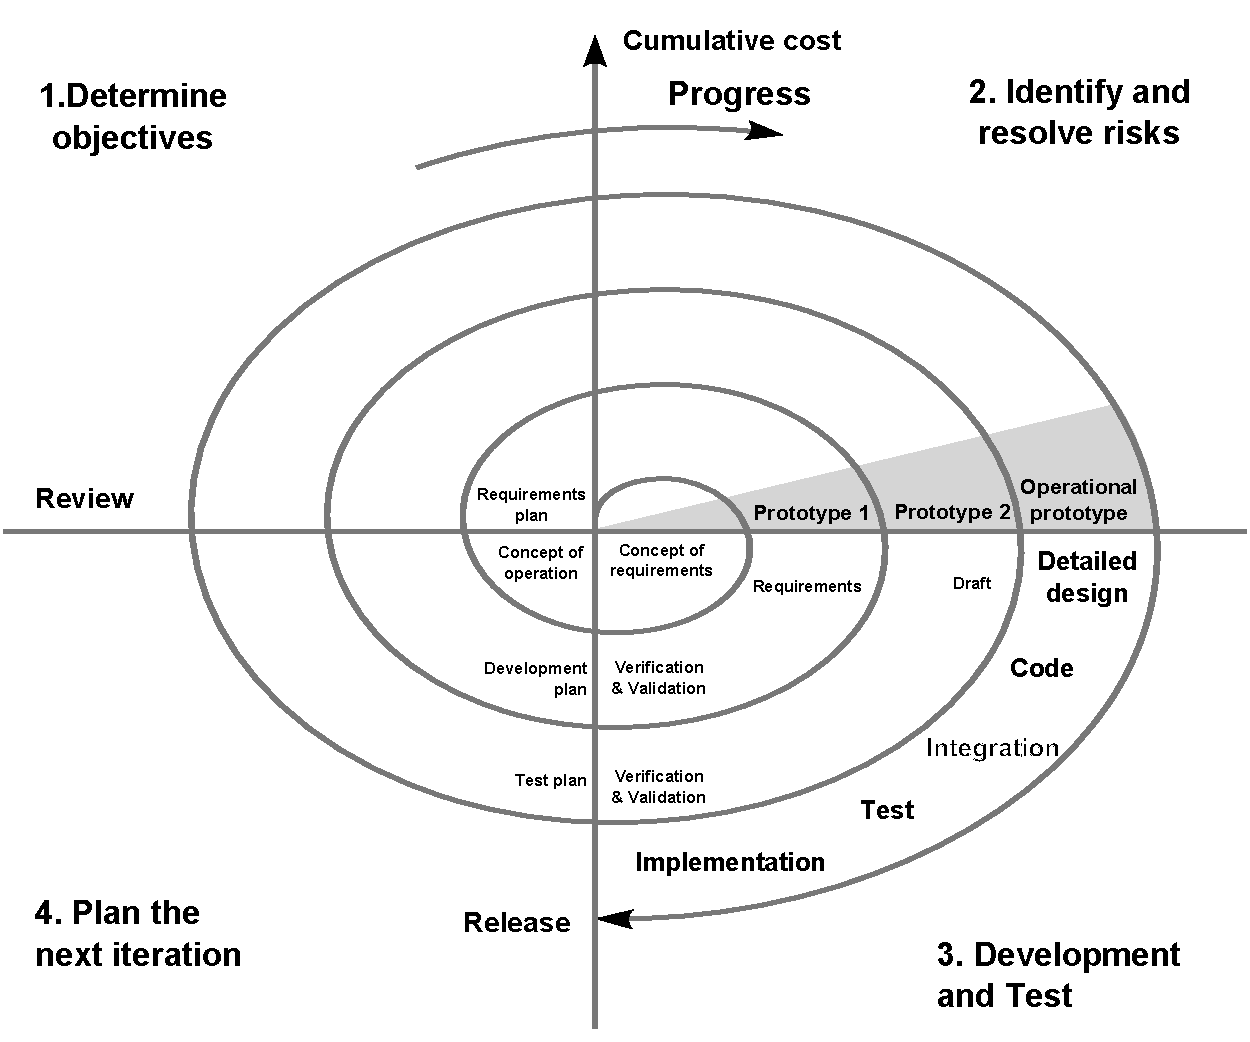
\includegraphics[width=0.58\textwidth]{Figures/Spiral_model.pdf}
	\caption{Spirálový model \cite{ee27bbyhk5LP1Ekm}}
	\label{fig:spiral-model}
\end{figure}

\newpage
\section{Testování API}
Předchůdcem API bylo vzdálené volání procedur (RPC), které vycházelo z potřeby zpracovávaní velkých dat či náročných komplexních výpočetních operací. V této době už k řešení zmíněných problémů nestačily procesory v osobních počítačích. Proto se zavedla metoda distribuovaných výpočtů, při kterých uživatelé výkon svých počítačů sdíleli. Možnost rozdělit úlohy na více částí se ale neobešla bez potíží. Například pokud někdo vypnul svůj počítač v době, kdy byl využíván ke vzdálenému zpracování úloh jiných uživatelů, mohlo dojít k tomu, že se proces vypnul, aniž by dokončil svou práci.

V dnešní době můžeme hovořit o dvou typech API. První možností je lokální aplikační rozhraní využívané například k interakci s operačními systémy nebo databázemi. Příkladem API operačního systému může být systémové volání pro čtení ze souboru. Tato systémová volání jsou programátorovi však skryta za funkcemi programovacích jazyků.

Z druhého pohledu na aplikační rozhraní se jedná o způsob propojení organizací či aplikací. Toto propojení může zajišťovat vzájemnou integraci. Strana využívající API tak nemusí implementovat své vlastní řešení, které již strana poskytující API vyřešila. Na straně druhé může dojít na straně poskytovatele API k chybě, v tomto případě může u strany využívající API dojít také k problémům, které je nutné řešit \cite{Mitchell2015}.


\section{Manuální a automatizované testování}
Testování softwaru je možné rozdělit do dvou základních skupin. Manuální testování zpravidla provádí člověk. Naopak automatizované testování zajišťuje stroj, který dle zvoleného scénáře většinou generuje požadavky na systém a čeká na odpověď, kterou porovnává s předpokládaným výstupem.

Automatizované testování nám může v krátkém čase přinést mnoho zajímavých výsledků. Dává nám náhled na to, na co se v daném systému zaměřit. Stojí však na poměrně náročném vytváření testových plánů či schémat. V případě nalezení chyby při automatickém testování se ale obvykle \\k problému musí dostat v posledním kroku i člověk, jehož úkolem je nalezení chyby v kódu. Využití automatizovaných testů je nesporně výhodné, především z časových důvodů, neboť můžeme stejné scénáře spouštět několikrát za sebou, např. s upravenými vstupy, které si můžeme nechat generovat. Výstupem automatizovaného testování je většinou souhrn či stručný přehled akcí, které se provedly. Tyto akce jsou pak označeny, zda se výstup rovná očekávanému výstupu. V případě projektu HEAppE Middleware jde o testování rozhraní REST API.

Automatizace testování je takřka nutností. Manuální techniky jednoduše neumožňují dostatečné testování ke zmírnění rizik, vzhledem k tomu, že jedno API samo o sobě může vyžadovat stovky testů, které je ve většině případů nutné opakovat \cite{Mitchell2015}.



\section{Framework pro automatizované testování HEAppE}
Mezi základní úkoly pro automatizované testování softwaru se řadí výběr frameworku\footnote{Framework je set programů, knihoven a rozhraní, které programátorovi zjednodušují práci. Framework většinou stačí nakonfigurovat a používat.}. Pro účely HEAppE Middleware byl vybrán Robot Framework \cite{UDdvJfGpGdOGQs2a}. Jedná se o automatizační Open-Source framework, který pracuje s vytvořenou provozuschopnou aplikací či API. Tento framework se využívá na úrovni integračního testování, v praxi jde o tzv. smoke testy \cite{K35ZsSqAfq3Ec1XJ}. Hlavním úkolem smoke testů je rychlé vyhodnocení funkčnosti aplikace, aby bylo možné přejít k dalšímu vývoji. Pomáhají odhalit nefunkční části aplikace či aplikačního rozhraní. Robot Framework je schopný pracovat \\s grafickým uživatelským rozhraním, ale pracuje i na úrovni REST API.

Robot Framework je nezávislý na operačním systému, jádro frameworku pak stojí na běhovém prostředí Python Interpreter\footnote{Python Interpreter převádí kód psaný v jazyce Python do jazyka strojových instrukcí, tyto instrukce jsou následně spouštěny a program v jazyce Python je vykonáván.}. To umožňuje především snadnou rozšiřitelnost a použitelnost. Základem automatizovaného testování prostřednictvím Robot Frameworku je sestavení testovacích plánů. Jedná se o popis akcí, které má framework vykonat. V případě HEAppE Midleware bude Robot Framework testovat endpointy REST API, pro dané požadavky pak budou dynamicky vytvářeny JSON specifikace. Základním plánem pro automatizované testování bude autentizace, vytvoření \\a spuštění úlohy. Tento plán může být dále rozšiřován.

Velkou výhodou tohoto frameworku je možné napojení na průběžnou integraci ve fázi vývoje. Průběžná integrace (Continuous Integration) slouží k urychlení nalezení chyb, integrace je spouštěna na integračním serveru podle předem zvoleného schématu. Metoda průběžné integrace je využívána i v projektu HEAppE, v průběhu sestavování aplikace je možné provést sadu testů z Robot Frameworku. Vývojáři pak budou mít lepší přehled o funkčnosti systému v dané fázi vývoje. Průběžná integrace je spouštěna předem nastavenou akcí. Může se například jednat o úpravu repositáře\footnote{Repositář je typ datové úložiště verzovacího systému.} či dané větve repositáře projektu. Sestavení a smoke testy jsou pak spouštěny automaticky, vývojář tak může sledovat stav integrace s informacemi o provedených testech. Metoda Continuous Integration je znázorněna na obrázku \ref{fig:ci}.

\begin{figure}[h]
	\centering
	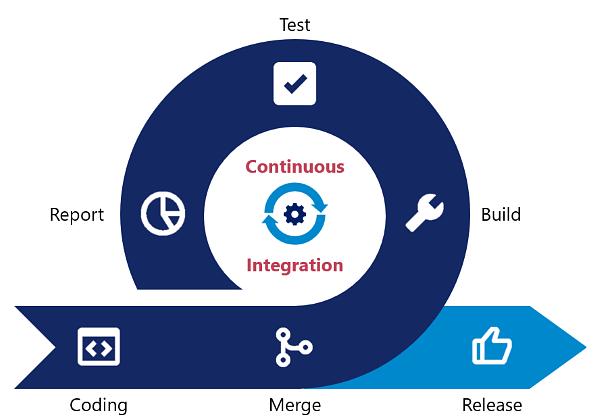
\includegraphics[width=0.6\textwidth]{Figures/cicd.png}
	\caption{Průběžná integrace \cite{cGNjWevJUlEHf7YF}}
	\label{fig:ci}
\end{figure}

\newpage
\section{Testovací scénář pro HEAppE}
Robot Framework je skvělým kandidátem pro testování hotových softwarových řešení. Pomocí tohoto frameworku je možné otestovat aplikační rozhraní daného systému z pohledu uživatele. Pro komplexní otestování HEAppE je možné vytvořit několik testovacích scénářů, které na sebe mohou navazovat. Základním scénářem pro používání HEAppE Middleware je vytvoření a spuštění úlohy na výpočetním clusteru. Z tohoto případu užití vychází i základní scénář pro automatizované testování HEAppE prostřednictvím Robot Framework.

Důležitým krokem při užívaní HEAppE Middleware je provedení autentizace. HEAppE po úspěšné autentizaci uživatele vrátí vygenerovaný unikátní identifikátor, který uživatel následně přidává do každé další žádosti při volání endpointu.

Hlavním úkolem tohoto testovacího plánu bude otestování spouštění úloh na výpočetních clusterech. Na každý cluster bude podána žádost o spuštění několika konfigurací úloh tak, aby byly otestovány všechny varianty specifikací úloh.

Součástí této práce je vytvoření testovacího plánu k otestování funkcionalit HEAppE při užívání rozšíření pro lokální spouštění úloh. Testovací plán taktéž bude testovat nově vytvořené endpointy v sekci Management, které jsou určené ke správě šablon výpočtů (Command Template).

\newpage
Před spouštěním úloh budou otestovány funkcionality související s uživatelem HEAppE. Tyto kroky se nachází v následující tabulce \ref{tab:user-testing}.

\begin{table}[!h]
	\centering
		\begin{tabular}{|C{0.8cm}|c|c|}
		    \hline
		    Krok & Název & Endpoint \\
		    \hline
			1 & Získání seznamu dostupných clusterů & \specialcell{/heappe/ClusterInformation/\\ListAvailableClusters}\\
			\hline
			2 & Autentizace uživatele & \specialcell{/heappe/UserAndLimitationManagement/\\
			AuthenticateUserPassword}\\
            \hline
			3 & \specialcell{Získání využití zdrojů a limity\\ uživatele HEAppE} & \specialcell{/heappe/\\UserAndLimitationManagement/\\GetCurrentUsageAndLimitationsForCurrentUser}\\
            \hline
            4 & \specialcell{Získání využití zdrojů na výpočetních \\clusterech} & 	\specialcell{/heappe/ClusterInformation/\\CurrentClusterNodeUsage}\\
            \hline
            5 & Získání využití zdrojů uživatele HEAppE & \specialcell{/heappe/JobReporting/\\GetUserResourceUsageReport}\\
            \hline
            6 & \specialcell{Získání využití zdrojů skupiny uživatelů\\HEAppE} & \specialcell{/heappe/JobReporting/\\GetUserGroupResourceUsageReport}\\
            \hline
		\end{tabular}
	\caption{Seznam kroků pro testování funkcionalit souvisejících s uživatelem HEAppE}
	\label{tab:user-testing}
\end{table}

Dále bude otestováno spouštění pěti různě specifikovaných úloh na superpočítačových clusterech s různými typy plánovačů. Kroky určené k otestování jedné úlohy popisují kroky uvedené v tabulce \ref{tab:task-testing}. 

Zmiňovaná pětice specifikací úloh obsahuje úlohy popsané v následujícím seznamu. Konfigurace těchto úloh byly popisovány výše v kapitole \ref{chapter:chapter-about-heappe-middleware}.

\begin{itemize}
    \item Základní úloha
    \item Úloha využívající generickou šablonu výpočtů
    \item Úloha se specifikací extrémně dlouhé úlohy
    \item Úloha využívající funkcionality JobArrays
    \item Úloha s definovanou závislostí na jiné úloze
\end{itemize}


\begin{table}[!h]
	\centering
		\begin{tabular}{|C{0.8cm}|C{6.9cm}|c|}
		    \hline
		    Krok & Název & Endpoint \\
		    \hline
			1 & Vytvoření úlohy & \specialcell{/heappe/JobManagement/CreateJob}\\
			\hline
			2 & Spuštění zpracování úlohy & \specialcell{/heappe/JobManagement/SubmitJob}\\
            \hline
			3 & \specialcell{Získání spotřebovaných zdrojů úlohy} & \specialcell{/heappe/JobReporting/\\GetResourceUsageReportForJob}\\
            \hline
            4 & \specialcell{Získání využití zdrojů na výpočetních \\clusterech} & 	\specialcell{/heappe/ClusterInformation/\\CurrentClusterNodeUsage}\\
            \hline
            5 & \specialcell{Získání stavu úlohy} & \specialcell{/heappe/JobManagement/GetCurrentInfoForJob}\\
            \hline
            6 & \specialcell{Vyčkání na spuštění úlohy} & \specialcell{/heappe/JobManagement/GetCurrentInfoForJob}\\
            \hline
            7 & \specialcell{Získání IP adres alokovaných uzlů} & \specialcell{/heappe/JobManagement/GetAllocatedNodesIPs}\\
            \hline
            8 & \specialcell{Zrušení úlohy} & \specialcell{/heappe/JobManagement/CancelJob}\\
            \hline
            9 & \specialcell{Vyčkání na ukončení úlohy} & \specialcell{/heappe/JobManagement/GetCurrentInfoForJob}\\
            \hline
            10 & \specialcell{Smazání úlohy} & \specialcell{/heappe/JobManagement/DeleteJob}\\
            \hline
		\end{tabular}
	\caption{Seznam kroků pro testování úloh HEAppE}
	\label{tab:task-testing}
\end{table}
\newpage

Provedením kroků, které se nacházejí v tabulce \ref{tab:task-testing-management}, se otestuje funkčnost již výše popsané správy Command Template. Implementace tohoto rozšíření HEAppE o správu Command Template je taktéž součástí této práce. Dle specifikace jsou Management endpointy dostupné jen uživateli HEAppE s rolí Administrátor.


\begin{table}[!h]
	\centering
		\begin{tabular}{|C{0.8cm}|C{6.9cm}|c|}
		    \hline
		    Krok & Název & Endpoint \\
		    \hline
			1 & Vytvoření Command Template & \specialcell{/heappe/Management/CreateCommandTemplate}\\
			\hline
			2 & Modifikace specifikace Command Template & \specialcell{/heappe/Management/ModifyCommandTemplate}\\
            \hline
			3 & \specialcell{Smazání Command Template} & \specialcell{/heappe/Management/\\RemoveCommandTemplate}\\
			\hline
		\end{tabular}
	\caption{Seznam kroků pro testování Management sekce HEAppE}
	\label{tab:task-testing-management}
\end{table}
\newpage

Protože je práce s úlohou na výpočetním clusteru řízena plánovačem, prakticky se jedná o předávání pokynů. Proto se v testovacím plánu musí vyskytovat čekání na vykonání příkazu. Při pokynu pro spuštění úlohy tak musíme čekat na to, až naši úlohu spustí plánovač na výpočetním clusteru. V testovacím scénáři je toto čekání implementováno opakovaným voláním HEAppE REST API s prodlevou, aby nedošlo k zablokování (toto chování by mohlo nést znaky DOS/DDOS útoku). Následuje ukázka kódu testovacího scénáře Robot Frameworku obsahujícího popsané cyklické volání REST API. V tomto případě se cyklus ukončí, pokud HEAppE vrátí stav, který značí, že je úloha spuštěna. Očekává se, že se stav změní v rámci jednotek či desítek minut, Robot Framework neumožňuje práci s cykly s neznámým počtem opakování. Proto byl při implementaci využit cyklus se známým počtem opakování, horní interval cyklu byl nastaven na maximální povolenou hodnotu.

Útržek testovacího scénáře obsahuje funkci WaitForJobRuns. Úkolem této funkce je počkat na spuštění úlohy plánovačem na výpočetním clusteru.


\lstinputlisting[language=bash, caption={Segment Robot Framework testu}]{SourceCodes/wait-for-job-runs.txt}

Výsledkem tohoto testování je vygenerovaný report a log. Programátor pak má lepší představu \\o funkčnosti jednotlivých částí systému. Tyto reporty Robot Framework připraví v grafické podobě. Dostupné jsou ve formátu html. Surová data jsou součástí reportu ve struktuře XML\footnote{Výměnný formát pro přenos dat}.




Test či testový plán může být prováděn pravidelně a několikrát za sebou. Počáteční časové náklady na sestavení tohoto scénáře jsou nesrovnatelné s přínosem, které automatizované testování přináší. Test navíc může běžet v pozadí automaticky a vývojář si tak jen vyzvedne výsledek.


Tento testovací scénář je možné volně rozšiřovat nebo vytvářet scénáře obdobné. Velmi praktické je i využití Robot Frameworku pro testování softwaru v době vývoje. Scénář můžeme měnit podle aktuálních požadavků např. při vývoji nové funkcionality.

Výše popsaný testový scénář byl použit k otestování funkčnosti HEAppE Middleware s užitím lokálního spouštění úloh na hostitelském počítači. Tímto byla prokázána validita implementovaných rozšíření, které popisuje tato práce. Pro uživatele je užití lokálního simulovaného clusteru prostřednictvím HEAppE takřka nerozeznatelné od použití HEAppE se skutečným výpočetním clusterem.

Navíc byly otestovány další endpointy, které je vhodnější testovat manuálně. Jedná se především \\o funkcionality HEAppE Middleware pro přenos dat, kdy je vhodnější provádět kontroly ručně.
Výsledky těchto automatizovaně prováděných testů jsou součástí práce v kapitole příloh v sekci \ref{chapter:robot-framework-local-tests}. 

Manuálně byly otestovány endpointy \emph{/heappe/FileTransfer/GetFileTransferMethod} a \emph{/heappe/FileTransfer/EndFileTransferMethod} za pomocí aplikace, která je součástí repositáře HEAppE. Tyto endpointy slouží k otevření přenosového kanálu mezi klientským počítačem a superpočítačovým clusterem. Funkcionalita tedy umožňuje přenos souborů mezi fyzickým počítačem uživatele \\a superpočítačovým clusterem. Při tomto testování byl otevřen přenosový kanál, pomocí protokolu SCP\footnote{Protokol sloužící k bezpečnému přenosu mezi dvěma počítači.} byl na cluster přesunut soubor, a následně byl přenosový kanál uzavřen. Výsledek tohoto testu se nachází v kapitole příloh v sekci \ref{manual-tests}.

